\chapter{Arquitetura e Modelagem do Sistema}

Este capítulo apresenta a arquitetura e modelagem do sistema de registro de ponto eletrônico desenvolvido, detalhando a estrutura organizacional do \textit{software}, as tecnologias empregadas, os padrões arquiteturais adotados e o modelo de dados implementado. O sistema foi concebido seguindo uma arquitetura distribuída, com separação clara entre \textit{frontend} e \textit{backend}, permitindo escalabilidade, manutenibilidade e flexibilidade na evolução da aplicação.

\section{Visão Geral da Arquitetura}

O sistema de registro de ponto eletrônico foi desenvolvido utilizando uma arquitetura em três camadas (3-tier), separando claramente as responsabilidades entre apresentação, lógica de negócio e persistência de dados. Esta abordagem segue os princípios da arquitetura SOA (\textit{Service-Oriented Architecture}) e REST (\textit{Representational State Transfer}), promovendo a interoperabilidade e facilitando a integração com sistemas externos.

A Figura~\ref{fig:arquitetura-geral} apresenta a visão geral da arquitetura do sistema, destacando os principais componentes e suas interações.

\begin{figure}[htbp]
\centering
\begin{tikzpicture}[
    node distance=1.5cm,
    box/.style={rectangle, draw, fill=blue!10, text width=3cm, text centered, minimum height=1.2cm},
    api/.style={rectangle, draw, fill=green!10, text width=2.5cm, text centered, minimum height=1cm},
    db/.style={cylinder, draw, fill=yellow!10, text width=2cm, text centered, minimum height=1.5cm, aspect=0.25},
    external/.style={rectangle, draw, fill=red!10, text width=2.5cm, text centered, minimum height=1cm},
    arrow/.style={->, thick}
]

% Frontend Layer
\node[box] (client) at (0,6) {Cliente Web\\(Next.js 15)};
\node[box] (auth) at (0,4) {Autenticação\\(NextAuth.js)};

% API Gateway
\node[api] (gateway) at (5,5) {API Gateway\\(NestJS)};

% Backend Services
\node[api] (auth-service) at (3,2.5) {Auth Service};
\node[api] (user-service) at (7,2.5) {User Service};
\node[api] (company-service) at (3,0.5) {Company Service};
\node[api] (point-service) at (7,0.5) {Point Service};

% Database
\node[db] (database) at (11,3) {PostgreSQL\\Database};

% External Services
\node[external] (maps) at (2,8) {Google Maps\\API};
\node[external] (geolocation) at (8,8) {Geolocation\\Services};

% Connections
\draw[arrow] (client) -- (gateway) node[midway, above] {HTTPS/REST};
\draw[arrow] (auth) -- (gateway);
\draw[arrow] (gateway) -- (auth-service);
\draw[arrow] (gateway) -- (user-service);
\draw[arrow] (gateway) -- (company-service);
\draw[arrow] (gateway) -- (point-service);
\draw[arrow] (auth-service) -- (database);
\draw[arrow] (user-service) -- (database);
\draw[arrow] (company-service) -- (database);
\draw[arrow] (point-service) -- (database);
\draw[arrow] (client) -- (maps);
\draw[arrow] (client) -- (geolocation);

\end{tikzpicture}
\caption{Arquitetura geral do sistema de registro de ponto}
\label{fig:arquitetura-geral}
\end{figure}

A arquitetura adotada proporciona as seguintes vantagens:

\begin{itemize}
    \item \textbf{Separação de Responsabilidades}: Cada camada possui responsabilidades bem definidas, facilitando a manutenção e evolução do sistema;
    \item \textbf{Escalabilidade}: A arquitetura permite escalar horizontalmente cada componente de forma independente;
    \item \textbf{Testabilidade}: A separação em camadas facilita a implementação de testes unitários e de integração;
    \item \textbf{Reutilização}: Os serviços do \textit{backend} podem ser consumidos por diferentes clientes;
    \item \textbf{Segurança}: A centralização da lógica de autenticação e autorização no \textit{backend} garante maior segurança.
\end{itemize}

\section{Modelagem de Dados}

O modelo de dados foi projetado seguindo os princípios da normalização de banco de dados e os padrões do Domain-Driven Design (DDD). O sistema utiliza PostgreSQL como sistema de gerenciamento de banco de dados, aproveitando suas características de robustez, conformidade com ACID e suporte a tipos de dados complexos.

A Figura~\ref{fig:modelo-entidades} apresenta o diagrama de classes UML do modelo de dados, destacando as principais entidades, seus atributos, métodos e relacionamentos.

\begin{figure}[htbp]
\centering
\resizebox{\textwidth}{!}{%
\begin{tikzpicture}[scale=0.4,every node/.style={transform shape}]

% Organização hierárquica com máximo espaçamento

% Nível 1: Entidade principal
\umlclass[x=8, y=20, width=1.5cm]{Empresa}{
    + id: UUID \\
    + nome: String \\
    + cnpj: String
}{
    + validarRaio(): Boolean
}

% Nível 2: Entidades dependentes da empresa  
\umlclass[x=0, y=14, width=1.5cm]{Departamento}{
    + id: UUID \\
    + nome: String \\
    + empresaId: UUID
}{
    + listarCargos(): Cargo[]
}

\umlclass[x=8, y=14, width=1.5cm]{Usuario}{
    + id: UUID \\
    + nome: String \\
    + email: String \\
    + papel: UserRole
}{
    + autenticar(): Boolean
}

\umlclass[x=16, y=14, width=1.5cm]{HorarioFuncionario}{
    + id: UUID \\
    + diaSemana: Integer \\
    + horarioInicio: Time
}{
    + calcularHoras(): Number
}

% Nível 3: Entidades específicas
\umlclass[x=0, y=8, width=1.5cm]{Cargo}{
    + id: UUID \\
    + nome: String \\
    + baseSalarial: Decimal
}{
    + calcularSalario(): Decimal
}

\umlclass[x=8, y=8, width=2cm]{InformacoesTrabalhistas}{
    + id: UUID \\
    + usuarioId: UUID \\
    + dataAdmissao: Date
}{
    + calcularTempo(): Number
}

% Nível 4: Entidades operacionais
\umlclass[x=4, y=2, width=1.8cm]{RegistroPonto}{
    + id: UUID \\
    + tipo: TipoRegistro \\
    + dataHora: DateTime \\
    + status: StatusRegistro
}{
    + validarSequencia(): Boolean
}

\umlclass[x=12, y=2, width=1.5cm]{Justificativa}{
    + id: UUID \\
    + motivo: String \\
    + tipo: TipoJustificativa
}{
    + aprovar(): void
}

% Relacionamentos UML
\umluniaggreg[arg1=empresas, mult1=1, pos1=0.2, arg2=usuarios, mult2=*, pos2=0.8]{Empresa}{Usuario}
\umluniaggreg[arg1=empresa, mult1=1, pos1=0.8, arg2=departamentos, mult2=*, pos2=0.2]{Empresa}{Departamento}
\umluniaggreg[arg1=departamento, mult1=1, pos1=0.8, arg2=cargos, mult2=*, pos2=0.2]{Departamento}{Cargo}
\umlcompo[arg1=usuario, mult1=1, pos1=0.2, arg2=informacoes, mult2=1, pos2=0.8]{Usuario}{InformacoesTrabalhistas}
\umluniassoc[arg1=informacoes, mult1=*, pos1=0.2, arg2=cargo, mult2=1, pos2=0.8]{InformacoesTrabalhistas}{Cargo}
\umluniassoc[arg1=informacoes, mult1=*, pos1=0.8, arg2=departamento, mult2=1, pos2=0.2]{InformacoesTrabalhistas}{Departamento}
\umluniaggreg[arg1=usuario, mult1=1, pos1=0.8, arg2=horarios, mult2=*, pos2=0.2]{Usuario}{HorarioFuncionario}
\umluniaggreg[arg1=usuario, mult1=1, pos1=0.2, arg2=registros, mult2=*, pos2=0.8]{Usuario}{RegistroPonto}
\umluniaggreg[arg1=registro, mult1=1, pos1=0.8, arg2=justificativas, mult2=*, pos2=0.2]{RegistroPonto}{Justificativa}

\end{tikzpicture}
}
\caption{Diagrama de classes UML do modelo de dados}
\label{fig:modelo-entidades}
\end{figure}

\subsection{Entidades Principais}

O modelo de dados é composto por oito entidades principais, organizadas hierarquicamente para atender aos requisitos funcionais do sistema:

\subsubsection{Empresa}

A entidade \texttt{Empresa} representa a organização central que utiliza o sistema. Esta entidade armazena informações corporativas essenciais, incluindo dados de identificação (nome, CNPJ, email), configurações de geolocalização (latitude, longitude, raio permitido) e políticas operacionais de tolerância para registros de ponto. A empresa serve como entidade agregadora para todos os demais componentes do sistema.

\subsubsection{Usuario}

A entidade \texttt{Usuario} modela os diferentes tipos de usuários do sistema: proprietários, administradores e funcionários. Implementa um sistema de controle de acesso baseado em papéis (RBAC - \textit{Role-Based Access Control}) através do campo \texttt{papel}, garantindo que cada usuário tenha acesso apenas às funcionalidades compatíveis com seu nível de autorização.

\subsubsection{Departamento}

A entidade \texttt{Departamento} representa as divisões organizacionais da empresa, permitindo uma estruturação hierárquica clara e facilitando o controle administrativo. Cada departamento pode conter múltiplos cargos e funcionários, proporcionando flexibilidade na organização interna.

\subsubsection{Cargo}

A entidade \texttt{Cargo} define as posições e funções específicas dentro da organização. Além das informações descritivas, armazena dados salariais base que servem como referência para cálculos de folha de pagamento e relatórios financeiros.

\subsubsection{InformacoesTrabalhistas}

A entidade \texttt{InformacoesTrabalhistas} consolida todos os dados contratuais do funcionário, incluindo data de admissão, período de início dos registros de ponto, carga horária semanal contratual e informações salariais. Esta entidade estabelece a ponte entre os dados pessoais do usuário e suas responsabilidades profissionais.

\subsubsection{HorarioFuncionario}

A entidade \texttt{HorarioFuncionario} modela os horários de trabalho individualizados, permitindo flexibilidade na definição de expedientes específicos por dia da semana. Suporta configurações de intervalos para refeições e diferentes jornadas de trabalho conforme as necessidades operacionais.

\subsubsection{RegistroPonto}

A entidade \texttt{RegistroPonto} armazena todos os registros de ponto dos funcionários, incorporando validação geográfica automática e controle rigoroso de status (aprovado, pendente, justificado). Cada registro inclui coordenadas GPS, timestamp preciso e indicadores de conformidade com as políticas empresariais.

\subsubsection{Justificativa}

A entidade \texttt{Justificativa} implementa um sistema completo de justificativas para registros irregulares, incluindo workflow de aprovação, categorização por tipos específicos e rastreabilidade completa do processo decisório. Permite que gestores analisem e aprovem/rejeitem justificativas de forma controlada.

\subsection{Relacionamentos e Cardinalidades}

Os relacionamentos entre as entidades seguem as regras de negócio do domínio:

\begin{itemize}
    \item Uma empresa pode ter múltiplos usuários, departamentos e configurações de horário (1:N);
    \item Cada usuário pertence a uma única empresa, mas pode ter múltiplos registros de ponto e horários (1:N);
    \item As informações trabalhistas mantêm relacionamento 1:1 com o usuário, garantindo integridade referencial;
    \item Registros de ponto podem ter múltiplas justificativas, permitindo rejeição e reenvio (1:N).
\end{itemize}

\section{Arquitetura do Back-End}

O \textit{backend} foi desenvolvido utilizando o \textit{framework} NestJS, que implementa os padrões arquiteturais do Angular para o ambiente Node.js. A escolha do NestJS se justifica pela robustez na implementação de APIs RESTful, suporte nativo a TypeScript, sistema de injeção de dependências e extensa capacidade de integração com bibliotecas do ecossistema Node.js.

\subsection{Estrutura Modular}

A arquitetura do \textit{backend} segue o padrão modular do NestJS, organizando funcionalidades em módulos coesos e fracamente acoplados. A Figura~\ref{fig:arquitetura-backend} ilustra a estrutura modular implementada.

\begin{figure}[htbp]
\centering
\begin{tikzpicture}[
    app/.style={rectangle, draw, fill=blue!20, text width=2.5cm, text centered, minimum height=1cm},
    module/.style={rectangle, draw, fill=green!15, text width=2cm, text centered, minimum height=0.8cm},
    db/.style={cylinder, draw, fill=yellow!15, text width=2cm, text centered, minimum height=1cm, aspect=0.25}
]

% Aplicação Principal
\node[app] (app) at (6,8) {\textbf{NestJS Application}\\(AppModule)};

% Módulos de Negócio
\node[module] (auth) at (0,5) {\textbf{Auth}\\Autenticação\\JWT};
\node[module] (users) at (4,5) {\textbf{Usuários}\\CRUD\\Gestão};
\node[module] (companies) at (8,5) {\textbf{Empresas}\\Configurações\\Geolocalização};
\node[module] (point) at (12,5) {\textbf{Ponto}\\Registros\\Justificativas};

% Banco de Dados
\node[db] (database) at (6,1) {\textbf{PostgreSQL}\\TypeORM};

% Conexões
\draw[->] (app) -- (auth);
\draw[->] (app) -- (users);
\draw[->] (app) -- (companies);
\draw[->] (app) -- (point);

\draw[->] (auth) -- (database);
\draw[->] (users) -- (database);
\draw[->] (companies) -- (database);
\draw[->] (point) -- (database);

\end{tikzpicture}
\caption{Arquitetura modular do backend NestJS}
\label{fig:arquitetura-backend}
\end{figure}

\subsection{Camadas Arquiteturais}

O \textit{backend} implementa uma arquitetura em camadas bem definidas:

\begin{description}
    \item[Camada de Apresentação (Controllers)] Responsável por receber e processar requisições HTTP, validar parâmetros de entrada e retornar respostas adequadas. Utiliza decoradores do NestJS para mapeamento de rotas e validação automática através das bibliotecas \texttt{class-validator} e \texttt{class-transformer}.
    
    \item[Camada de Negócio (Services)] Concentra a lógica de negócio da aplicação, implementando regras específicas do domínio como validação de geolocalização, cálculo de banco de horas e workflows de aprovação de justificativas.
    
    \item[Camada de Acesso a Dados (Repositories)] Implementada através do TypeORM, fornece abstração para operações de persistência, mapeamento objeto-relacional e gerenciamento de transações.
    
    \item[Camada de Segurança (Guards e Middlewares)] Implementa autenticação JWT, autorização baseada em papéis e validações de segurança transversais.
\end{description}

\subsection{Principais Funcionalidades}

O \textit{backend} implementa as seguintes funcionalidades principais:

\begin{itemize}
    \item \textbf{Autenticação e Autorização}: Sistema completo baseado em JWT com refresh tokens e controle de sessão;
    \item \textbf{Gestão de Usuários}: CRUD completo com validação de dados e controle de status;
    \item \textbf{Controle de Ponto}: Registro com validação geográfica, sequenciamento obrigatório e cálculo automático de horas;
    \item \textbf{Sistema de Justificativas}: Workflow completo com aprovação/rejeição e rastreabilidade;
    \item \textbf{Relatórios}: Cálculo de banco de horas, extração de dados e relatórios gerenciais.
\end{itemize}

\section{Arquitetura do Front-End}

O \textit{frontend} foi desenvolvido utilizando Next.js 15 com React 19, aproveitando as funcionalidades avançadas de Server-Side Rendering (SSR), Static Site Generation (SSG) e o novo App Router. Esta escolha tecnológica proporciona excelente performance, SEO otimizado e experiência de usuário superior.

\subsection{Estrutura de Componentes}

A aplicação segue os padrões de design de componentes do React, implementando uma arquitetura baseada em componentes reutilizáveis e contextualizada. A Figura~\ref{fig:arquitetura-frontend} apresenta a estrutura organizacional do \textit{frontend}.

\begin{figure}[htbp]
\centering
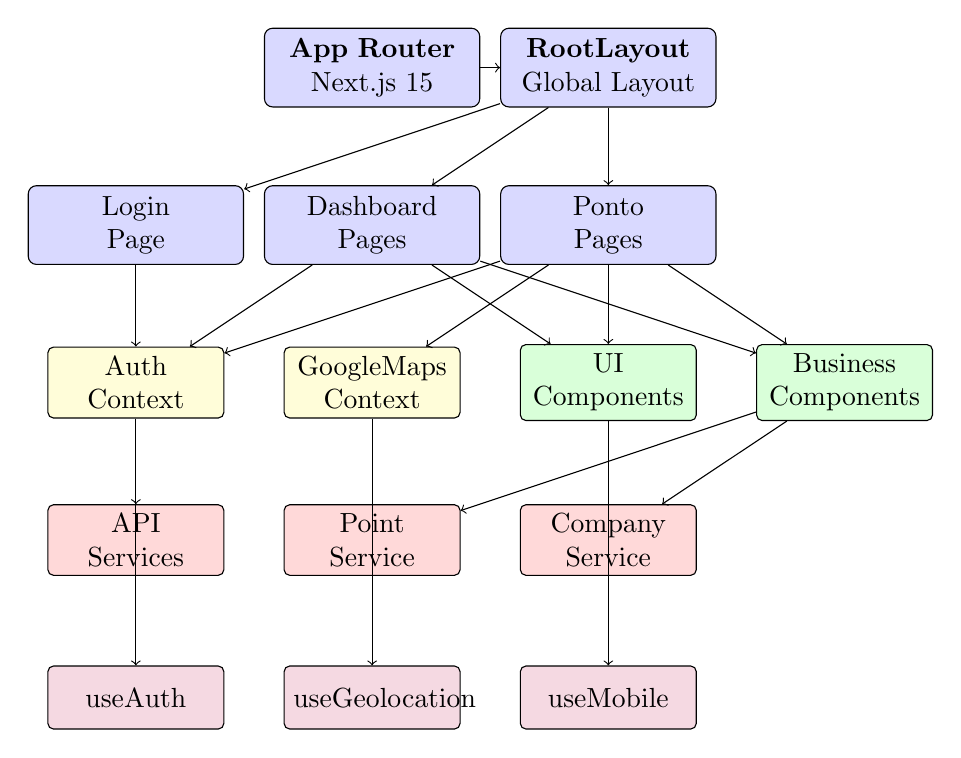
\begin{tikzpicture}[
    page/.style={rectangle, draw, fill=blue!15, text width=2.5cm, text centered, minimum height=1cm, rounded corners=3pt},
    component/.style={rectangle, draw, fill=green!15, text width=2cm, text centered, minimum height=0.8cm, rounded corners=2pt},
    context/.style={rectangle, draw, fill=yellow!15, text width=2cm, text centered, minimum height=0.8cm, rounded corners=2pt},
    service/.style={rectangle, draw, fill=red!15, text width=2cm, text centered, minimum height=0.8cm, rounded corners=2pt},
    hook/.style={rectangle, draw, fill=purple!15, text width=2cm, text centered, minimum height=0.8cm, rounded corners=2pt}
]

% App Structure
\node[page] (app) at (0,8) {\textbf{App Router}\\Next.js 15};
\node[page] (layout) at (3,8) {\textbf{RootLayout}\\Global Layout};

% Pages
\node[page] (login) at (-3,6) {Login\\Page};
\node[page] (dashboard) at (0,6) {Dashboard\\Pages};
\node[page] (ponto) at (3,6) {Ponto\\Pages};

% Contexts
\node[context] (auth-ctx) at (-3,4) {Auth\\Context};
\node[context] (maps-ctx) at (0,4) {GoogleMaps\\Context};

% Components
\node[component] (ui-comp) at (3,4) {UI\\Components};
\node[component] (business-comp) at (6,4) {Business\\Components};

% Services
\node[service] (api-service) at (-3,2) {API\\Services};
\node[service] (point-service) at (0,2) {Point\\Service};
\node[service] (company-service) at (3,2) {Company\\Service};

% Custom Hooks
\node[hook] (auth-hook) at (-3,0) {useAuth};
\node[hook] (geo-hook) at (0,0) {useGeolocation};
\node[hook] (mobile-hook) at (3,0) {useMobile};

% Connections
\draw[->] (app) -- (layout);
\draw[->] (layout) -- (login);
\draw[->] (layout) -- (dashboard);
\draw[->] (layout) -- (ponto);

\draw[->] (login) -- (auth-ctx);
\draw[->] (dashboard) -- (auth-ctx);
\draw[->] (ponto) -- (auth-ctx);
\draw[->] (ponto) -- (maps-ctx);

\draw[->] (dashboard) -- (ui-comp);
\draw[->] (dashboard) -- (business-comp);
\draw[->] (ponto) -- (ui-comp);
\draw[->] (ponto) -- (business-comp);

\draw[->] (auth-ctx) -- (api-service);
\draw[->] (business-comp) -- (point-service);
\draw[->] (business-comp) -- (company-service);

\draw[->] (auth-ctx) -- (auth-hook);
\draw[->] (maps-ctx) -- (geo-hook);
\draw[->] (ui-comp) -- (mobile-hook);

\end{tikzpicture}
\caption{Arquitetura de componentes do frontend Next.js}
\label{fig:arquitetura-frontend}
\end{figure}

\subsection{Padrões Arquiteturais Implementados}

O \textit{frontend} implementa diversos padrões arquiteturais modernos:

\begin{description}
    \item[Component-Based Architecture] Toda a interface é construída através de componentes React reutilizáveis, seguindo os princípios de Single Responsibility e composição.
    
    \item[Context API] Implementação de contextos globais para autenticação, configurações de mapas e estado da aplicação, evitando prop drilling e centralizando estados compartilhados.
    
    \item[Custom Hooks] Encapsulamento de lógicas complexas em hooks customizados, promovendo reutilização e separação de responsabilidades.
    
    \item[Service Layer] Abstração das chamadas de API através de serviços especializados, facilitando manutenção e testes.
    
    \item[Design System] Implementação de um sistema de design consistente utilizando Radix UI e Tailwind CSS, garantindo acessibilidade e responsividade.
\end{description}

\subsection{Gerenciamento de Estado}

O gerenciamento de estado da aplicação utiliza uma abordagem híbrida:

\begin{itemize}
    \item \textbf{Estado Local}: Componentes individuais gerenciam seus estados internos através do hook \texttt{useState};
    \item \textbf{Estado Global}: Contextos React para dados compartilhados (autenticação, configurações);
    \item \textbf{Estado do Servidor}: React Query (TanStack Query) para cache e sincronização de dados remotos;
    \item \textbf{Estado de Formulários}: React Hook Form para validação e gerenciamento eficiente de formulários.
\end{itemize}

\section{Fluxo de Autenticação e Autorização}

O sistema implementa um fluxo de autenticação robusto baseado em JWT (\textit{JSON Web Tokens}) com integração entre \textit{frontend} e \textit{backend}. A Figura~\ref{fig:fluxo-auth} ilustra o processo completo de autenticação.

\begin{figure}[htbp]
\centering
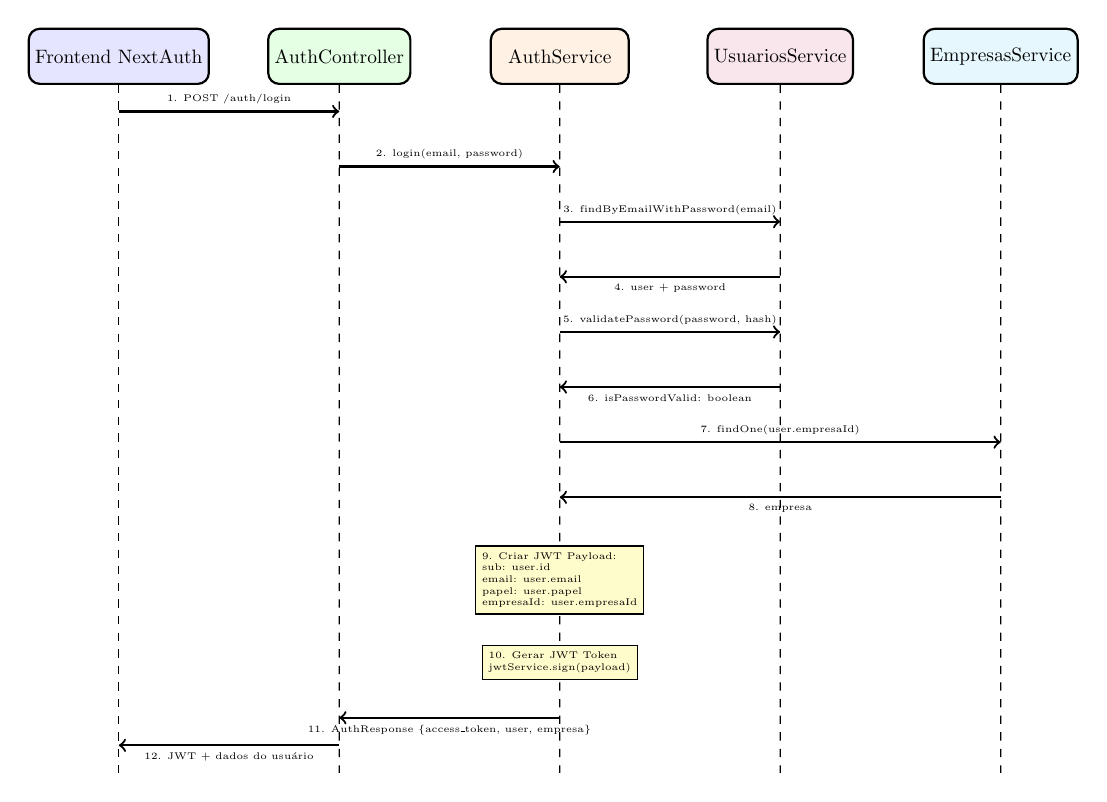
\begin{tikzpicture}[scale=0.7, every node/.style={transform shape}]
    % Participantes
    \node[draw, rounded corners, thick, fill=blue!10, minimum width=2.5cm, minimum height=1cm] (client) at (0,12) {Frontend NextAuth};
    \node[draw, rounded corners, thick, fill=green!10, minimum width=2.5cm, minimum height=1cm] (auth) at (4,12) {AuthController};
    \node[draw, rounded corners, thick, fill=orange!10, minimum width=2.5cm, minimum height=1cm] (service) at (8,12) {AuthService};
    \node[draw, rounded corners, thick, fill=purple!10, minimum width=2.5cm, minimum height=1cm] (users) at (12,12) {UsuariosService};
    \node[draw, rounded corners, thick, fill=cyan!10, minimum width=2.5cm, minimum height=1cm] (company) at (16,12) {EmpresasService};

    % Linhas de vida
    \draw[dashed] (client) -- (0,-1);
    \draw[dashed] (auth) -- (4,-1);
    \draw[dashed] (service) -- (8,-1);
    \draw[dashed] (users) -- (12,-1);
    \draw[dashed] (company) -- (16,-1);

    % Mensagens do fluxo de autenticação
    \draw[->, thick] (0,11) -- node[above, font=\tiny]{1. POST /auth/login} (4,11);
    \draw[->, thick] (4,10) -- node[above, font=\tiny]{2. login(email, password)} (8,10);
    \draw[->, thick] (8,9) -- node[above, font=\tiny]{3. findByEmailWithPassword(email)} (12,9);
    \draw[<-, thick] (8,8) -- node[below, font=\tiny]{4. user + password} (12,8);
    \draw[->, thick] (8,7) -- node[above, font=\tiny]{5. validatePassword(password, hash)} (12,7);
    \draw[<-, thick] (8,6) -- node[below, font=\tiny]{6. isPasswordValid: boolean} (12,6);
    \draw[->, thick] (8,5) -- node[above, font=\tiny]{7. findOne(user.empresaId)} (16,5);
    \draw[<-, thick] (8,4) -- node[below, font=\tiny]{8. empresa} (16,4);

    % Processamento interno no AuthService
    \node[draw, fill=yellow!20, align=left, font=\tiny] at (8,2.5) {9. Criar JWT Payload:\\sub: user.id\\email: user.email\\papel: user.papel\\empresaId: user.empresaId};

    \node[draw, fill=yellow!20, align=left, font=\tiny] at (8,1) {10. Gerar JWT Token\\jwtService.sign(payload)};

    \draw[<-, thick] (4,0) -- node[below, font=\tiny]{11. AuthResponse \{access\_token, user, empresa\}} (8,0);
    \draw[<-, thick] (0,-0.5) -- node[below, font=\tiny]{12. JWT + dados do usuário} (4,-0.5);
\end{tikzpicture}
\caption{Diagrama de sequência - fluxo de autenticação}
\label{fig:fluxo-auth}
\end{figure}

\subsection{Componentes de Segurança}

O sistema de segurança é composto pelos seguintes elementos:

\begin{description}
    \item[JWT Strategy] Implementação da estratégia Passport.js para validação de tokens JWT no \textit{backend};
    \item[NextAuth.js] Biblioteca de autenticação para Next.js que gerencia sessões, tokens e callbacks;
    \item[Guards] Implementação de guards NestJS para proteção de rotas e validação de permissões;
    \item[Middleware] Middleware Next.js para proteção de rotas do \textit{frontend} baseado em papéis;
    \item[RBAC] Sistema de controle de acesso baseado em papéis com três níveis: funcionário, administrador e proprietário.
\end{description}

\subsection{Validação de Geolocalização}

Um dos diferenciais do sistema é a validação automática de geolocalização para registros de ponto. O processo utiliza a API de Geolocalização do navegador integrada com o Google Maps API para validação de presença física no local de trabalho.

O algoritmo de validação geográfica segue os seguintes passos:

\begin{enumerate}
    \item \textbf{Obtenção da localização}: Captura das coordenadas GPS do dispositivo do funcionário
    \item \textbf{Busca da localização da empresa}: Recuperação das coordenadas cadastradas da empresa
    \item \textbf{Cálculo de distância}: Aplicação da fórmula de Haversine para determinar a distância precisa
    \item \textbf{Validação do raio}: Verificação se a distância está dentro do raio permitido
    \item \textbf{Definição do status}: Aprovação automática ou solicitação de justificativa conforme configuração
\end{enumerate}

O algoritmo implementa a fórmula de Haversine para cálculo preciso de distância entre coordenadas geográficas, considerando a curvatura da Terra. A validação permite configuração flexível de raio de tolerância por empresa e políticas diferenciadas para registros fora da área permitida.